\chapter{La régulation}

\section{Introduction}
La réalisation du système nécessite une régulation de courant imbriquée dans une régulation de position. Le schéma suivant illustre cette architecture :

\begin{figure}[H]
    \centering
    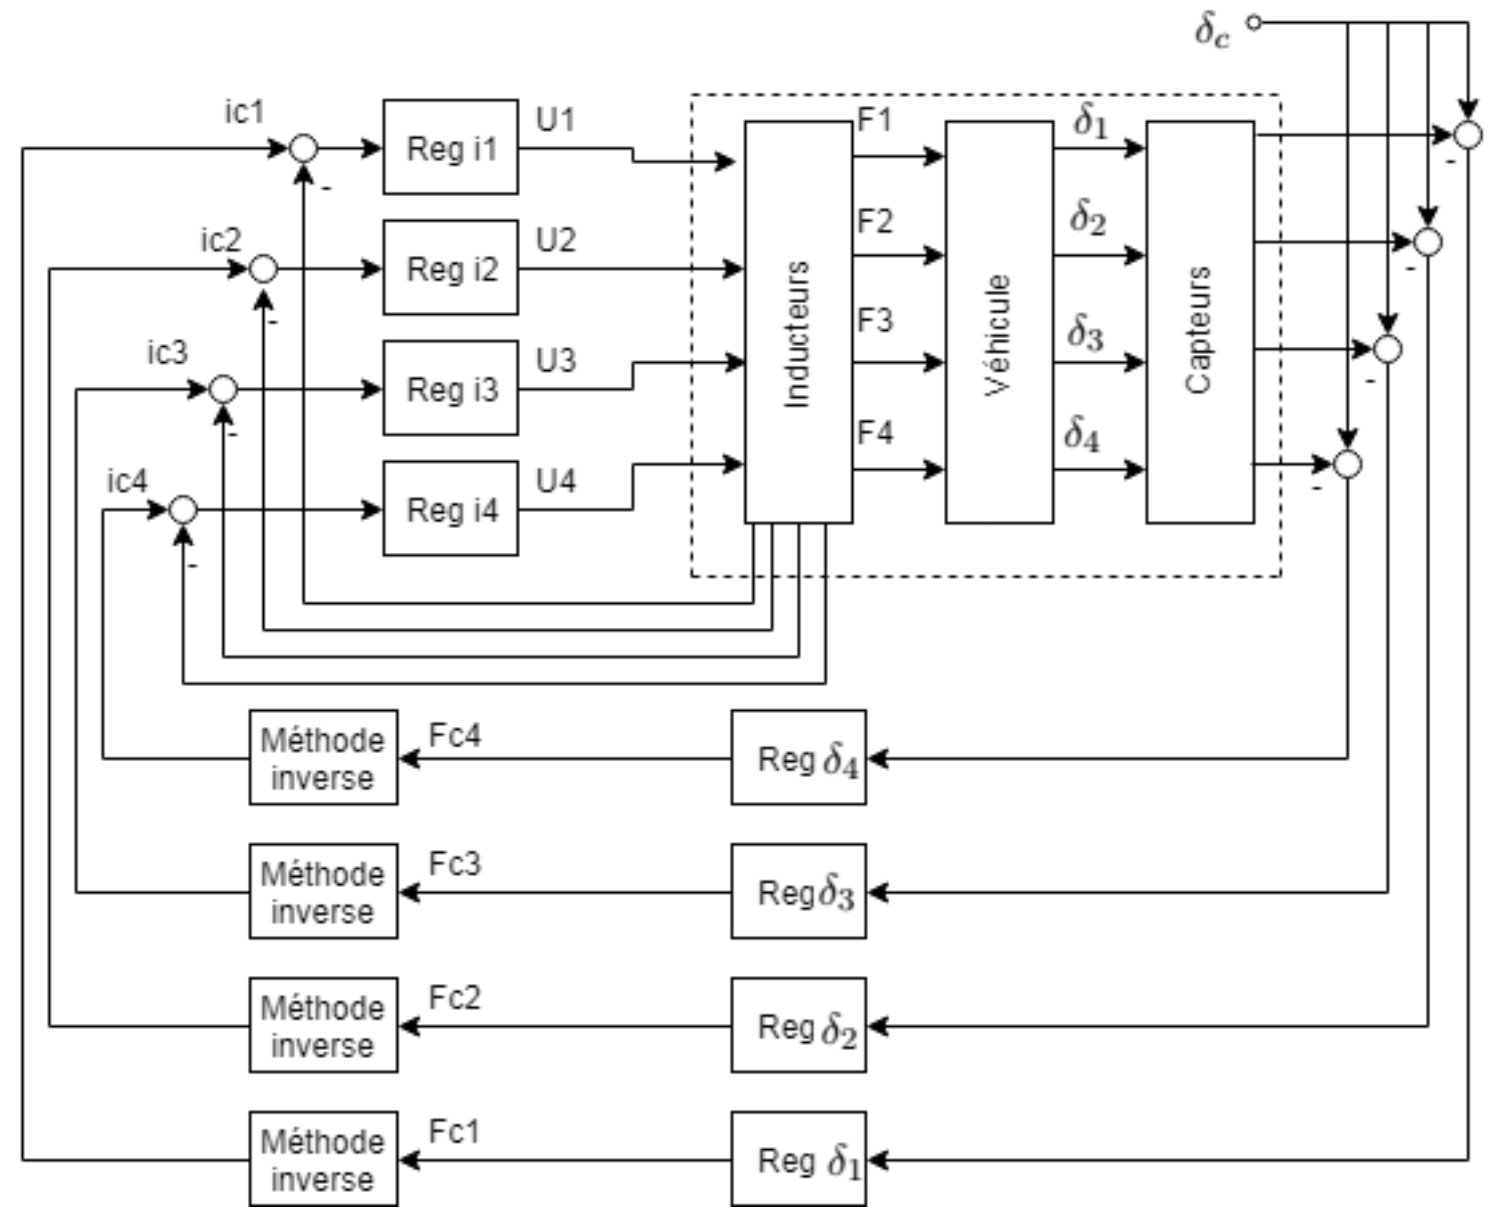
\includegraphics[width=0.8\linewidth]{Image/Chap.2/SchemaBlocRegulation.jpg}
    \caption{Schéma bloc de la régulation de courant imbriquée position \cite{Laucella}}
    \label{fig:SchemaBlocRégulation}
\end{figure}

Cette disposition permet d'assurer la lévitation de la maquette. La régulation de courant assure le contrôle du courant traversant l'inducteur, tandis que la régulation de position détermine l'élévation de la maquette par la mesure de la distance de l'entrefer.

Les blocs "Reg i1" à "Reg i4" représentent la régulation de courant. Un courant de consigne est fourni en entrée et une tension est appliquée aux inducteurs en sortie. Cette régulation de courant est réalisée par un régulateur PI.

Les blocs "Reg $\delta$1" à "Reg $\delta$4" représentent la régulation de position. Celle-ci reçoit une position en entrée et génère une force en sortie. Ce contrôle est assuré par une régulation par retour d'état (espace d'état).

Les blocs « méthode inverse » ont pour but de calculer le courant à partir de l'équation de la force émise par un électroaimant \ref{eq:ForceElectro} :

\begin{equation}
    F = k \cdot \left(\frac{I}{d}\right)^2
    \label{eq:ForceElectro}
\end{equation}

Avec :
\begin{itemize}
    \item $F$ : La force magnétique [N].
    \item $k$ : La constante de l'électroaimant [$\text{N}\cdot\text{m}^2/\text{A}^2$].
    \item $d$ : La distance de l'entrefer [m].
    \item $I$ : Le courant traversant la bobine [A].
\end{itemize}

À partir de cette relation, il est possible d'extraire le courant à induire dans la bobine en l'isolant selon l'équation \ref{eq:CourantElectro} :

\begin{equation}
    I = \sqrt{\frac{F}{k}} \cdot d
    \label{eq:CourantElectro}
\end{equation}

\section{Définition du système}

\subsection{Le système}
Le système garde la même définition que les travaux précédents qui représenté par la figure \ref{}

Pour rappel, voici les différentes grandeurs présentes dans la maquette :

\begin{table}[H]
    \centering
    \renewcommand{\arraystretch}{1.2}
    \begin{tabular}{|c|l|c|c|}
        \hline
        \multicolumn{4}{|c|}{\textbf{Paramètres Mécaniques}}                                                  \\ \hline
        \textbf{Symbole} & \textbf{Description de la grandeur}             & \textbf{Valeur} & \textbf{Unité} \\ \hline
        $m_{tot}$        & Masse totale du chariot (actuelle)              & 18.052          & kg             \\ \hline
        $m$              & Masse supportée par 1 inducteur ($m_{tot} / 4$) & 4.513           & kg             \\ \hline
        $g$              & Accélération gravitationnelle                   & 9.81            & m/s$^2$        \\ \hline
        $d$              & Distance entre 2 inducteurs (même essieu)       & 0.26            & m              \\ \hline
        $l$              & Distance entre 2 inducteurs (même rail)         & 0.28            & m              \\ \hline
    \end{tabular}
    \caption{Paramètres mécaniques de la maquette de sustentation.}
    \label{tab:param_mecaniques}
\end{table}

\begin{table}[H]
    \centering
    \renewcommand{\arraystretch}{1.2}
    \begin{tabular}{|c|l|c|c|}
        \hline
        \multicolumn{4}{|c|}{\textbf{Paramètres de l'Inducteur et de l'Entrefer}}                                                           \\ \hline
        \textbf{Symbole}             & \textbf{Description de la grandeur}                          & \textbf{Valeur}      & \textbf{Unité} \\ \hline
        $N$                          & Nombre de spires de la bobine                                & 125                  & -              \\ \hline
        $R$                          & Résistance de la bobine                                      & 0.8                  & $\Omega$       \\ \hline
        $A$                          & Surface de l'entrefer ($20 \text{ mm} \times 50 \text{ mm}$) & $1 \cdot 10^{-3}$    & m$^2$          \\ \hline
        $\mu_0$                      & Perméabilité du vide                                         & $4\pi \cdot 10^{-7}$ & H/m            \\ \hline
        $\delta_n$                   & Entrefer nominal (consigne)                                  & 2                    & mm             \\ \hline
        $\delta_{max}$ ou $\delta_0$ & Entrefer maximum (chariot posé)                              & 3                    & mm             \\ \hline
        $\delta_{min}$               & Entrefer minimum (structure collée)                          & 0.1                  & mm             \\ \hline
        $U_{dc}$                     & Tension d'alimentation du bus DC (PWM)                       & 48                   & V              \\ \hline
    \end{tabular}
    \caption{Paramètres électriques de l'inducteur et caractéristiques de l'entrefer.}
    \label{tab:param_inducteur_entrefer}
\end{table}

\begin{table}[H]
    \centering
    \renewcommand{\arraystretch}{1.2}
    \begin{tabular}{|c|l|c|c|}
        \hline
        \multicolumn{4}{|c|}{\textbf{Paramètres Numériques et Fréquences}}                                      \\ \hline
        \textbf{Symbole} & \textbf{Description de la grandeur}               & \textbf{Valeur} & \textbf{Unité} \\ \hline
        $f_e$            & Fréquence d'échantillonnage et de la PWM          & 25              & kHz            \\ \hline
        $T_e$ ou $h$     & Période d'échantillonnage ($1 / f_e$)             & 40              & $\mu$s         \\ \hline
        $f_{md}$         & Bande passante du capteur de position (Baumer)    & 1.1             & kHz            \\ \hline
        $f_{mi}$         & Fréquence de coupure retenue pour capteur courant & 25              & kHz            \\ \hline
    \end{tabular}
    \caption{Paramètres d'échantillonnage, traitement numérique et fréquences de coupure.}
    \label{tab:param_numeriques_frequences}
\end{table}

Afin d'alléger les calculs, les hypothèses suivantes ont été émise :

\begin{itemize}
    \item Perméance du fer infinie
    \item Pas de saturation du fer
    \item Effets de franges négligés
    \item Effet d’hystérésis négligé
    \item Flux de fuites négligés.
\end{itemize}

\subsection{Equation de la tension induite dans une bobine}

\subsection{Equation de Newton}

\subsection{Linéarisation des equations}

\section{La régulation de courant}

Donc si je comprends bien le problème avec une marge de phase aussi grande c'est qu'il faudrait des tension réelle de malade pour corriger rapidement la chose. La raison pour laquelle le 1.88 fonctionne c'est car il est faible et laisse suffisament de temps a mon circuit d'appliquer des tensions plus douces. Mais je peux "augmenter" la vitesse en allant en tatonemment de ma valeur de 1.88 jusqu'à une certaines valeurs max.

Concernant votre idée d'augmenter la vitesse par tâtonnement, c'est un grand OUI ! C'est d'ailleurs une démarche d'ingénierie extrêmement pertinente pour optimiser un système limité par son matériel.

\section{La régulation de position}